\documentclass[journal]{IEEEtran}

\usepackage{cite}

\usepackage{graphicx}  
%Please change to your image storage
\graphicspath{{../../Photos/member_photos/}}
\DeclareGraphicsExtensions{.pdf,.jpeg,.png}



\hyphenation{op-tical net-works semi-conduc-tor}


\begin{document}

\title{An Introduction to Our SAR Group Members}

%++++++++++++++++++++++++
\author{Wenhao~Hong\orcidlink{0000-0002-7394-5561},~\IEEEmembership{Postgraduate,~XDU,}
        Feixiang~Liu\orcidlink{0000-0003-3601-444X},~\IEEEmembership{Postgraduate,~XDU,}
        Feng~Wang\orcidlink{0000-0002-3089-7934},~\IEEEmembership{Postgraduate,~XDU,}
        and~Renjun~Luo\orcidlink{0000-0001-5903-481X},~\IEEEmembership{Postgraduate,~XDU}% <-this % stops a space
}


%++++++++++++++++++++++++
% The paper headers
\markboth{Operational Statistics for SAR Analysis}{Operational Statistics for SAR Analysis}




% make the title area
\maketitle

% As a general rule, do not put math, special symbols or citations
% in the abstract or keywords.
\begin{abstract}
	This paper is a brief group introduction to our SAR group members, which consists of our names, photos, characteristics, research interests as well as our respective ORCID Identifiers. Through the guidance of Prof.\ Frery, and by using the IEEE official template, we have completed this report.
\end{abstract}

% Note that keywords are not normally used for peerreview papers.
\begin{IEEEkeywords}
IEEE, Git Repository, Member Introduction
\end{IEEEkeywords}




\IEEEpeerreviewmaketitle



\section{Introduction}

%++++++++++++++++++++++++

\IEEEPARstart{C}reating a simple and perspicuous repository for a scientific project is a quite essential ability when performing scientific research. Therefore, we built our own git repository under the guidance of Prof. Frery~\cite{2020A}.
As is required by professor, we need to add our information including our names, personalities, photos as well as ORCID Identifiers to our newly built repository.
As a result, we submit a \LaTeX\ file into the repository with the information of each member in our group.

%+++++++++++++++++++++
\section{team member}

Wenhao Hong, from Jiangxi, has a lively personality and a wide range of interests. He likes to travel, listen to music and socialize. He does enjoy playing badminton, and often plays with friends during his free time. He loves to help others and once was a volunteer for the 14th Chinese National Games, dressing up as a mascot to entertain others and to obtain happiness himself.

Liu Feixiang, from Handan City, Hebei Province, likes to read, sing, love to learn, sunny, optimistic, and kind to people. During his undergraduate studies, he won the university-level scholarship for four consecutive years and participated in the innovation and entrepreneurship competition and won the provincial award. He is currently a graduate student of Professor Zhang Xiangrong.

Feng Wang, from Sichuan, likes playing badminton, loves sports, is outgoing and actively participates in various activities. He used to be a counselor assistant, deputy secretary of the third undergraduate branch of the AI Institute, and now is a postgraduate counselor of the AI Institute, with rich experience in student work. He studied actively and was successfully promoted as a postgraduate of Professor Xiangrong Zhang. 

Luo Renjun, a graduate student of the School of Artificial Intelligence, Class of 2022, studied in the School of Artificial Intelligence, Xi'an University of Electronic Science and Technology, and was guaranteed to continue his master's degree in the team of Professor Zhang Xiangrong in the School of Artificial Intelligence.

\bibliographystyle{unsrt}
%change it into your path
\bibliography{../Reference/reference_report1}


\begin{IEEEbiography}[{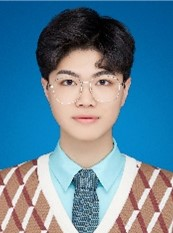
\includegraphics[width=1in,height=1.25in,clip,keepaspectratio]{wenhao.jpg}}]{Wenhao Hong}
(Postgraduate,~XDU) received his Bachelor of Engineering degree in Materials Science and Engineering from Xidian University in 2022, and won the second prize in the National English Competition for College Students in 2019. His current research interests are knowledge graph and object classification. 
\end{IEEEbiography}


 \begin{IEEEbiography}[{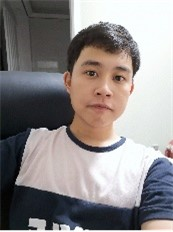
\includegraphics[width=1in,height=1.25in,clip,keepaspectratio]{feixiang.jpg}}]{Feixiang Liu}
(Postgraduate, XDU) received a bachelor's degree from the School of Artificial Intelligence of Xidian University in 2022, won the second prize at the provincial level of the 2021 National College Students Mathematics Competition, and won several university-level scholarships. His research interests are in three-dimensional reconstruction. 
\end{IEEEbiography}

  \begin{IEEEbiography}[{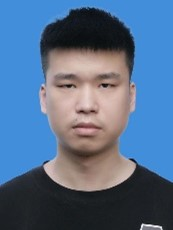
\includegraphics[width=1in,height=1.25in,clip,keepaspectratio]{wangfeng.jpg}}]{Feng Wang}
(Postgraduate, XDU) has won the excellent graduate students of Xidian University in 2020 and 2021, the first prize of Shaanxi Mathematical Contest in 2020, and the first prize of Shaanxi Mathematical Modeling Contest in 2020. Now the research direction is the detection application of knowledge graph. 
 \end{IEEEbiography}

 \begin{IEEEbiography}[{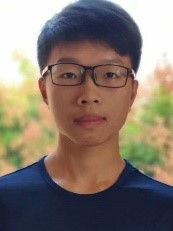
\includegraphics[width=1in,height=1.25in,clip,keepaspectratio]{renjun.jpg}}]{Renjun Luo}
(Postgraduate,~XDU) won scholarships for four consecutive years during his undergraduate studies, and was awarded the title of Outstanding Student of Xidian University in 2021, the International First Prize in the 2020 US Student Mathematical Modelling Competition, and the First Prize in the 2020 Shaanxi Provincial Mathematical Modelling Competition. His research interests are remote sensing target tracking and detection. 
\end{IEEEbiography}


\end{document}


